\documentclass[11pt,reqno,final]{amsart}

\pdfcompresslevel=0
\pdfobjcompresslevel=0

\usepackage[dvipsnames]{xcolor}% adds colors
\usepackage{amsmath, amsthm}% {amsfonts, amssymb}

% New Characters
\usepackage[latin1]{inputenc}%
\usepackage[T1]{fontenc}

\usepackage{MnSymbol}
\usepackage[normalem]{ulem}% underlining

\usepackage[theoremfont, largesc]{newpxtext} % different text,math font
\usepackage{newpxmath}

\makeatletter
\DeclareMathRadical{\sqrtsign}{symbols}{112}{largesymbols}{112}
% \let\sqrt=\undefined
% \DeclareRobustCommand\sqrt{\@ifnextchar[\@sqrt{\mathpalette\@x@sqrt}]}
% \def\@x@sqrt#1#2{%
%  \setbox\z@\hbox{$\m@th#1\sqrtsign{\mkern1mu #2}$}
%  \mkern3mu\box\z@}
\makeatother




% Page Typesetting
\usepackage[final]{microtype}
\usepackage{relsize}
\usepackage[margin=1in]{geometry}
\usepackage{framed}
\usepackage{tikz}

\usepackage{setspace}
\onehalfspacing

\usepackage{hyperref}
\hypersetup{
  final,
  pdftitle={Math 135 - The derivative and graphs},
  pdfauthor={Bonventre}, 
  linktoc=page,
  pagebackref,
  colorlinks=true,
  citecolor=PineGreen,
  linkcolor=PineGreen,
  linkbordercolor=PineGreen,
}


% Internal References

\usepackage[inline,shortlabels]{enumitem}

% \numberwithin{equation}{section} 
\numberwithin{figure}{section}

\usepackage[nameinlink,capitalise,noabbrev]{cleveref}

\crefname{equation}{}{} % get \cref to behave as \eqref

% \theoremstyle{plain} % bold name, italic text
\newtheorem{theorem}[equation]{Theorem}%
\newtheorem*{theorem*}{Theorem}%
\newtheorem{lemma}[equation]{Lemma}%
\newtheorem{proposition}[equation]{Proposition}%
\newtheorem{corollary}[equation]{Corollary}%
\newtheorem{conjecture}[equation]{Conjecture}%
\newtheorem*{conjecture*}{Conjecture}%
\newtheorem{claim}[equation]{Claim}%
\newtheorem{question}{Question}

\theoremstyle{definition} % bold name, plain text
\newtheorem{definition}[equation]{Definition}%
\newtheorem*{definition*}{Definition}%
\newtheorem{example}[equation]{Example}%
\newtheorem*{example*}{Example}%
\newtheorem{remark}[equation]{Remark}%
\newtheorem{notation}[equation]{Notation}%
\newtheorem{convention}[equation]{Convention}%
\newtheorem{assumption}[equation]{Assumption}%
\newtheorem{exercise}[question]{Exercise}

% ---------- macros
\newcommand{\set}[1]{\left\{#1\right\}}%
\newcommand{\sets}[2]{\left\{ #1 \;|\; #2\right\}}%
\newcommand{\longto}{\longrightarrow}%
\newcommand{\into}{\hookrightarrow}%
\newcommand{\onto}{\twoheadrightarrow}%

\usepackage{harpoon}
\newcommand{\vect}[1]{\text{\overrightharp{\ensuremath{#1}}}}

\newcommand{\del}{\partial}%

\newcommand{\ki}{\chi}
\newcommand{\ksi}{\xi}
\newcommand{\Ksi}{\Xi}

\newcommand{\dlim}{\displaystyle\lim}

% %%%%%%%%%%%%%%%%%%%%%%%%%%%%%%%%%%%%%%%%%%%%%%%%%%%%%%%%%%%%%%%%%%%%%%%%%%%%%%%%%%%%%%%%%%%%%%%%%%%%

\begin{document}

\newgeometry{bottom=0in}


\begin{center}
        \textbf{\Large Math 135, Calculus 1, Fall 2020}\\[10pt]
        {\large 10-07: The Derivative and Graphs}
\end{center}

\thispagestyle{empty}


\renewcommand{\thesection}{\Alph{section}}

% \vspace{-1pt}

Last time we introduced the \textbf{derivative} $f'(a)$ of a function $f(x)$ at the point $x=a$:
\begin{itemize}
\item the slope of the tangent line at $x=a$
\item the instantaneous velocity at time $x = a$
\item $\dlim_{h \to 0}\dfrac{f(a+h) - f(a)}{h}$
\end{itemize}

\begin{exercise}
        Let $f(x) = 3x^2 - x$.
        Find $f'(-2)$ by choosing the correct next step from each row below.
        In the third column, explain why this is the correct step, and what caused the error in the incorrect step.

        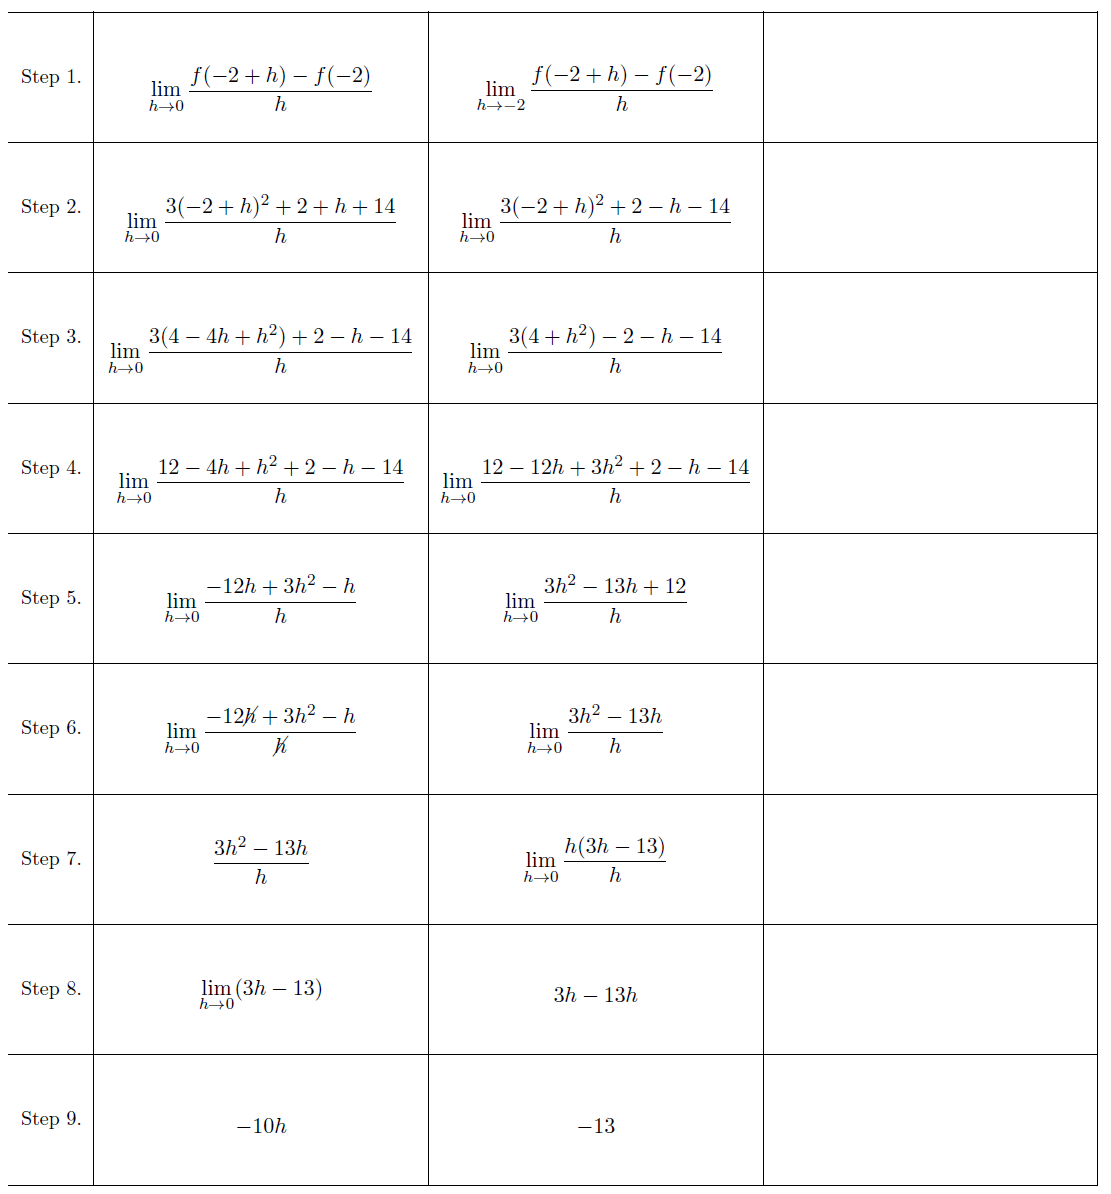
\includegraphics[width=1.1\textwidth]{10-07P_e1.png}
\end{exercise}

\newpage
\restoregeometry

\begin{exercise}
        Suppose that $g(x) = |x-3|$. Find $g'(2)$, $g'(3)$, and $g'(4)$.
        Draw a graph of $g$ and try to make sense of your answers.
        \textit{Hint: recall the definition of $|x-3|$ as a piecewise function. Where might your need to look at one-handed limits?}
        \vfill
\end{exercise}

\setcounter{section}{1}
\section{Deriative as a function}

If we let $a$ vary, the derivative $f'(a)$ is a \textbf{new function}.
\begin{definition}
        The \textbf{derivative} of $f(x)$ is the function $f'(x) = \dlim_{h \to 0}\dfrac{f(x+h) - f(x)}{h}$,
        with domain wherever this limit exists.
\end{definition}

\begin{framed}
        \begin{itemize}
        \item $f'(a) > 0$ exactly when $f(x)$ is \textbf{increasing} at $x=a$
        \item $f'(a) < 0$ exactly when $f(x)$ is \textbf{decreasing} at $x=a$
        \end{itemize}
\end{framed}

\begin{exercise}
        Suppose the following is the graph of the \textbf{derivative} $g'(x)$ of some function $g(x)$.
        Where is $g(x)$ increasing? Decreasing? Constant?
        
        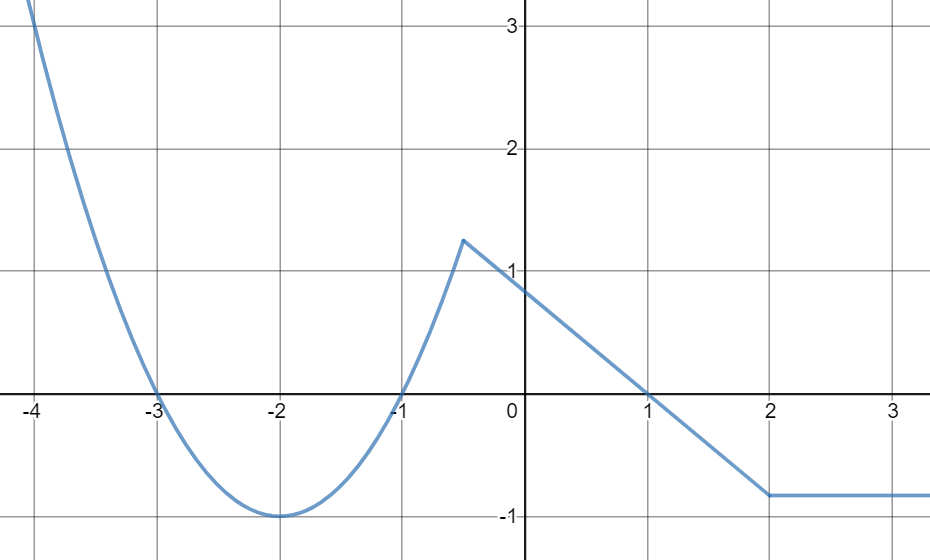
\includegraphics[width=2.7in]{10-07P_fprime.png}
\end{exercise}

\begin{exercise}
        Suppose $f(x)$ is the function with the following graph.
        Sketch the graph of $f'(x)$.
        \begin{minipage}{0.5\textwidth}
                \begin{center}
                        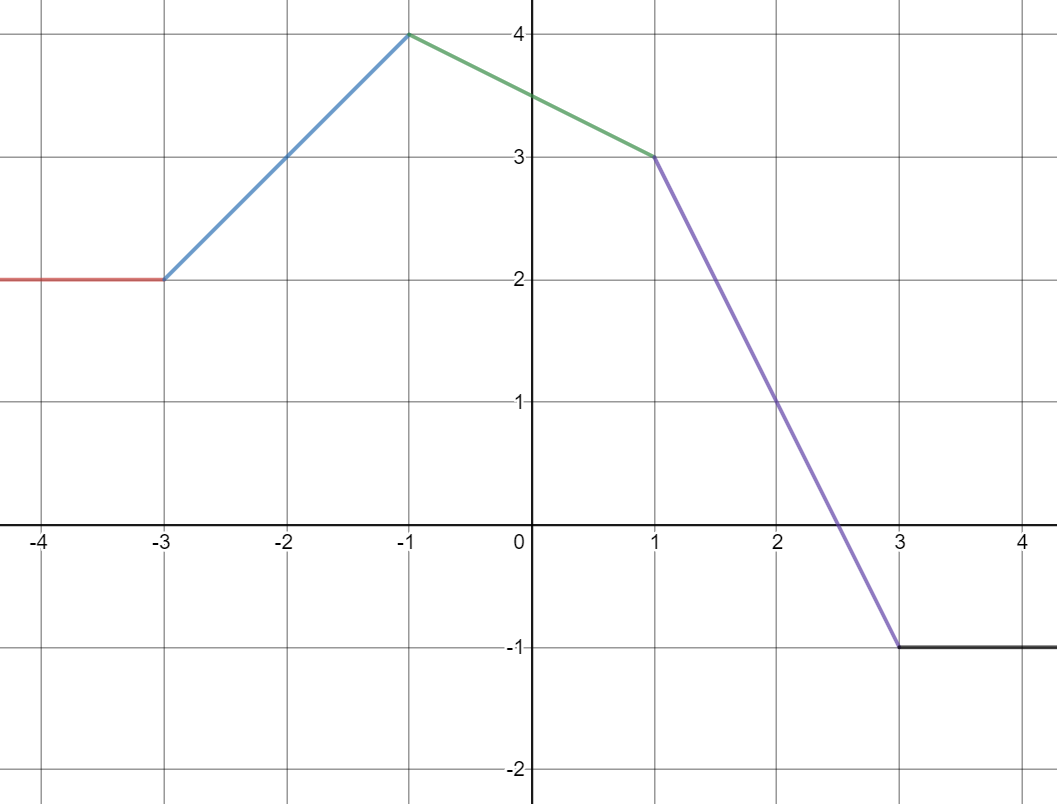
\includegraphics[width=2.5in]{10-07P_f.png}
                \end{center}
        \end{minipage}
        \begin{minipage}{0.5\textwidth}
                \begin{center}
                        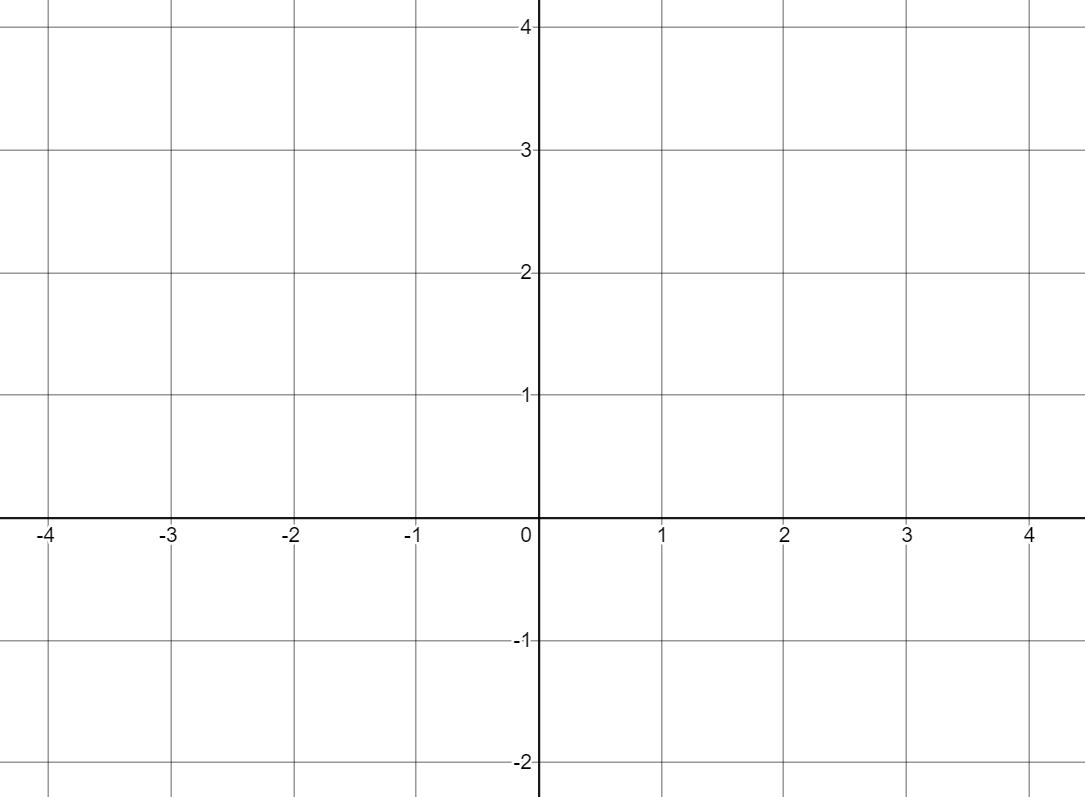
\includegraphics[width=2.5in]{10-07P_axes.png}
                \end{center}
        \end{minipage}
        
\end{exercise}

\end{document}
